\section{Colors}

Color coding is a fundamental aspect of computer graphics, dictating how colors displayed on-screen are represented as sequences of binary digits.
Typically, on-screen colors are encoded using the RGB system, which stands for Red-Green-Blue.

\subsection{Physical phenomena}
In terms of physics, the color of light is determined by the wavelength of the photons it emits.
When a light source emits photons of various wavelengths, objects interact with these photons based on their composition, either reflecting or absorbing them at different intensities.
The wavelengths of reflected photons contribute to the primary colors of an object.
These reflected photons are then focused by the lens of the human eye onto the retina, where specialized cells called rods and cones reside.
Rods are sensitive to light intensity, while cones are sensitive to light color.
Through these cells, the brain processes visual information. 
There are three distinct types of cones distributed evenly across the retina, each responsive to a specific portion of the light spectrum. 
The brain integrates signals from these cones to perceive a given color.

\begin{figure}[H]
    \centering
    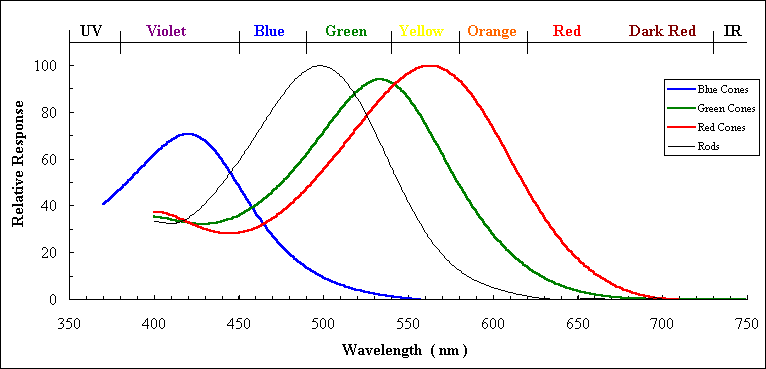
\includegraphics[width=0.4\linewidth]{images/cones.png}
    \caption{Human cones wavelength}
\end{figure}

\subsection{Color reproduction}
Color reproduction operates on the principle inverse to human vision, employing distinct emitters for each color perceptible by specific types of cones in the eye.
As the wavelengths perceived by the three types of cones primarily correspond to red, green, and blue, different hues are created by blending the light from these three primary colors. 
When observing a display from a sufficient distance, the human eye naturally blends the primary hues, reproducing the stimuli associated with a combined color.

By mixing two of the three primary colors, such as red and green or blue and red, we produce secondary colors like yellow, cyan, or magenta. 
Mixing all three primaries yields white, while adjusting the proportions of the three colors enables the reproduction of various hues.

Comparing the wavelengths of photons sensed by cones with the frequency spectrum helps understand why cyan results from blending blue and green, and yellow emerges from mixing red and green. 
The visible spectrum to the human eye is broad, characterized by a parabolic shape.

\begin{figure}[H]
    \centering
    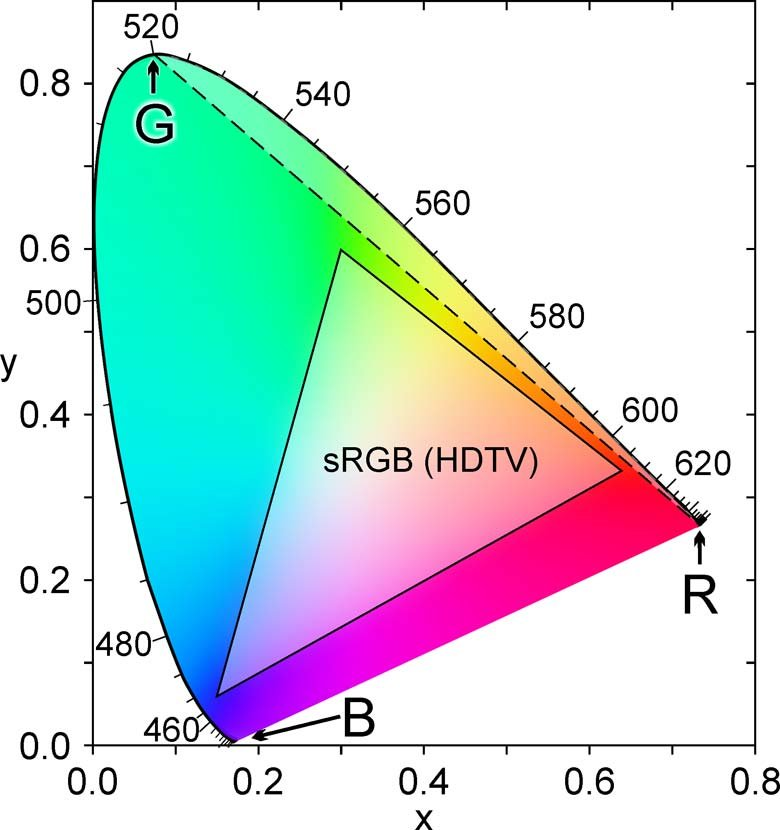
\includegraphics[width=0.35\linewidth]{images/range.png}
    \caption{Colors perceived by human eyes and reproduced by a monitor}
\end{figure}

The range of colors that a monitor can display corresponds to a cube, with the red, green, and blue components positioned along the $x$, $y$ and $z$-axis, respectively.

The levels of these components translate into electrical signals that regulate the intensity of light emitted by the screen for each primary color. 
In digital systems, these signals are typically generated through DAC (Digital-to-Analog Converter) conversion, resulting in quantization, which reduces the number of available colors.

Different monitors may assign various frequencies of the spectrum to each primary color and encode their levels differently. 
Color profiles are used to compensate for these variations, ensuring consistent behavior across different adapters.